\section{Variantendiskussion}
\label{sec:Variantendiskussion}
Zu Beginn soll eine Marktrecherche durchgeführt werden, um bestehende Lösungen zu analysieren und auf Eignung zu Prüfen. Mit den gewonnen Erkenntnissen soll dann abgewägt werden ob Standartsoftware beschafft werden kann oder eine eigenentwicklung Veranlasst wird.

Für die Entwicklung sollen verschidedene Architekturansätze vorgestellt und verglichen werden um so eine Entscheidung für ein vorgehen zu treffen werden das dann im Entwurf und der Implementation Umgesetzt werden kann.
%Das erfolgt im Rahmen einer Variantendiskussion, in der verschiedene Ansätze und Technologien zur Umsetzung der Software bewertet werden.

\subsection{Marktrecherche}
\label{sec:Marktrecherche}
Im Rahmen der Marktrecherche wurden drei verschiedene Softwarelösungen für die Anwesenheitsplanung verglichen. Das Ziel dieser Analyse war es, Akquisitionsoptionen für das geplante Softwareprojekt zu ermitteln. Um Entscheidungen über die Eignung treffen zu können, wurden die Softwareprodukte auf den Erfüllungsgrad ausgewählter Anforderungen geprüft und mit einer Bewertungsmatrix bewertet, die funktionale- und nichtfunktionale Anforderungen beinhaltete. Dabei wurden die Auswahlkriterien so gewählt und gewichtet das zwingend erforderliche Anforderungen höher gewichtet wurden als optionale Anforderungen.

%TODO:Tabelle muss ordentlich Platziert werden
\begin{table}[htbp]
    \centering
    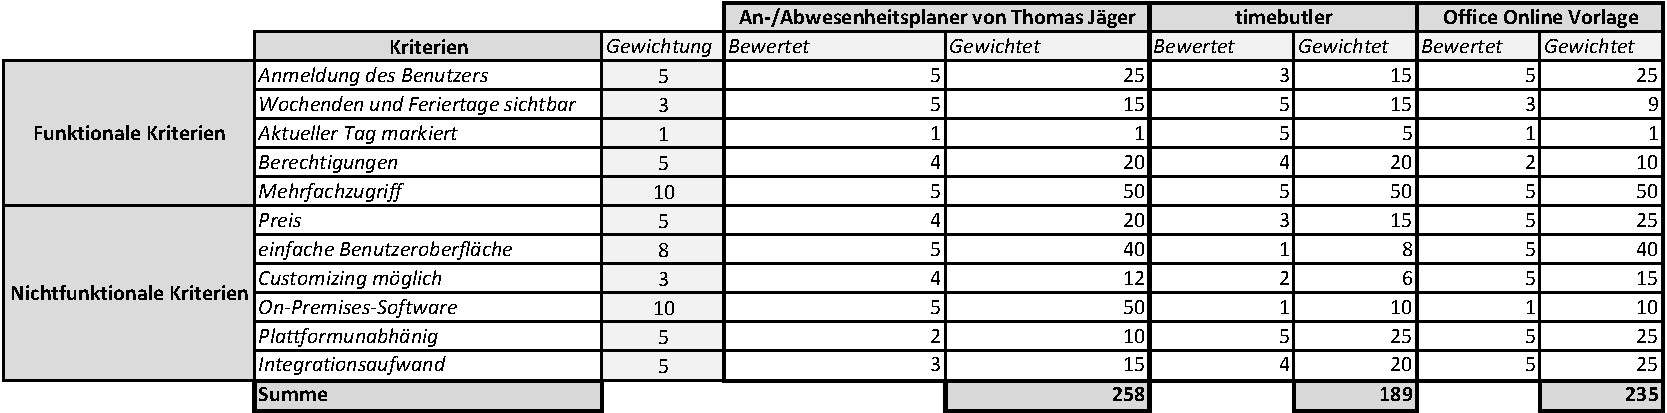
\includegraphics[width=0.9\textwidth,angle=0]{abb/Markterkundung.pdf}
    \caption[Beschreibung]{ Tabelle Markterkundung}
    \label{tab:Markterkundung}
\end{table}

\subsubsection{An-/Abwesenheitsplaner von Thomas Jäger}
\label{sec:AnAbwesenheitsplaner}
Die erste betrachtete Software, der An-/Abwesenheitsplaner von Thomas Jäger, zeichnete sich durch die besonders intuitive Benutzeroberfläche aus. Bei der Betrachtung der anderen funktionalen Kriterien wurde festgestellt, dass die Software alle benötigten Anforderungen erfüllt und damit für den Einsatz geeignet ist. Negativ zu bewerten ist allerding, das die Software nur als Windows Programm zur Verfügung steht und damit nicht Plattformunabhängig eingesetzt werden kann. Zudem müsste ein solches Programm auf jedem Client PC im SMK installiert werden um die Software für alle Nutzbar zu machen. Damit ergibt sich ein hoher initialer Integrationsaufwand und auch späterer Wartungsaufwand den es zu berücksichtigen gilt. (vgl. \cite{AnAbwesenPlaner})


%Die Benutzerfreundlichkeit wurde jedoch als etwas komplex und steil eingestuft, was eine gewisse Einarbeitungszeit erforderte. Zudem war der Support nur eingeschränkt verfügbar und die Preisgestaltung vergleichsweise hoch. (vgl. \cite{AnAbwesenPlaner})
\subsubsection{timebutler}
\label{sec:timebutler}
Das zweite Programm namens timebutler überzeugte hingegen durch seine Plattformunabhängigkeit. Damit könnte es ohne großen Integrationsaufwand im SMK eingeführt und betrieben werden. Die Software bietet alle geforderten Funktionalitäten hat jedoch eine komplizierte Benutzeroberfläche und stellt viele Funktionen bereit die nicht benötigt werden. Das resultiert in höheren Anschaffungskosten als bei dem An-/Abwesenheitsplaner von Thomas Jäger. Besonders negativ ist zu bewerten, dass die Software zwar Plattformunabhängig ist, da sie auf Webtechnologien aufbaut, jedoch nicht als On-Premises-Software verfügbar ist. Damit müsste auf die Cloud des Anbieters zurückgegriffen werden was nicht gewünscht ist. (vgl. \cite{timebutler})

\subsubsection{Online Office Datei}
\label{sec:OnlineOffice}
Die dritte betrachtete Lösung ist die Verwendung einer Online Tabellenkalkulations Vorlage. Das würde es ermöglichen, die bereits vorhandenen Excel Tabellen für die Anwesenheitsplanung weiter zu verwenden. Durch das zurückgreifen auf Online Funktionalitäten die \zB von Microsoft mit Office356 oder mit Onlyoffice in Verbindung mit Nextcloud zur Verfügung stehen, kann man den gleichzeitigen Zugriff auf diese Listern erreichen. Damit würde man das Hauptproblem der einfachen Excel Dateien lösen. Doch auch hier müsste man im Falle des einsatzes von Office356 auf die Microsoft Cloud zurückgreifen. Desweiteren gibt es nur begrenzte Möglichkeit diese Excel Listen vor ungewollter Änderungen zu schützen und ein Berechtigungskonzept durchzusetzten.

\subsubsection{Auswertung der Marktrecherche}
\label{sec:AuswertungMarktrecherche}
Nach Betrachtung der drei Programme wurde festgestellt, dass keines der drei für eine Akquisition in frage kommt, da jedes seine individuellen Schwachstellen mit sich bringt. Der An-/Abwesenheitsplaner von Thomas Jäger wäre von allen die beste Option, da es eine benutzerfreundliche Oberfläche, eine solide Funktionalität und eine angemessene Preisgestaltung vereint. Die Plattformunabhängigkeit ist jedoch im SMK ein großer Faktor, da sich das neue Programm möglichst gut in die vorhandene Infrastruktur einfügen soll. Deswegen wurde sich gegen eine Akquisition von Standartsoftware entschieden, um die geforderten Funktionalitäten zu erfüllen ohne dabei die Schwachstellen der Analysierten Programme inkauf nehmen zu müssen wurde die Eigenentwicklung der Software an Referat 12 übergeben.

\subsection{Eigenentwicklung}
\label{sec:Eigenentwicklung}

Durch die Eigenentwicklung sollen die spezifischen Anforderungen des SMK präzise Erfüllt und so Kompromisse und Funktionslücken wie bei den verglichenen Programmen vermieden werden. Die Flexibilität und Anpassungsfähigkeit einer Eigenentwicklung ermöglicht eine perfekte Integration mit bestehenden Systemen im SMK. Durch den Entwurf einer eigenen Benutzeroberfläche soll eine intuitive und benutzerfreundliche Lösung wie bei Excel den Umstieg er Mitagrbeiter verbessern, was spätere Schulungen vereinfacht. Darüber hinaus füher die Eigenentwicklung zur Möglichkeit der internen Wartung und Aktualisierung. Im nachhinein könnten einfache Funktionsupdates hinzugefügt werden um das Anwesenheitsplanungssystem weiterzuentwickeln. Ducht die Abaolute kontrolle über die Entwickelte Software können Datenschutz- und Datensicherheitsaspekte durch individuell implementierte Sicherheitsmaßnahmen getroffenwerden.

Bei einer Eigenentwicklung ist jedoch zu beachten, dass wie bei jedem Projekt Risiken wie zu hoher Zeitaufwand oder fehlendes Fachwissen vorhanden sind.


\subsection{Umsetzungsvarianten}
\label{sec:Umsetzungsvarianten}


\subsubsection{Benutzerinteraktionsmuster}
\label{sec:Benutzerinteraktionsmuster}
Nach eingehender Analyse der Anforderungen und der Markterkundung sollen verschiedene Umsetzungsvarianten für das geplante Softwareprojekt des Anwesenheitsplaners untersucht werden. Dabei sollen auf bestehende Entwurfsmuster zurückgegriffen und passende ausgewählt werden. Für die Benutzerinteraktion könnte auf das bewährte Model-View-Controller (MVC) Entwurfsmuster zurückgegriffen werden. Dieses Muster ermöglicht die getrennte Entwicklung von Model (Daten und Logik) und Benutzeroberfläche. Die Model Komponente implementiert alle funktionen die mit Dateninteraktion und Geschäftslogik einher gehen. Die View- und die Controllerkomponente sind dann für alle Benutzerinteraktionen und Visualisierungsaufgaben zuständig. Der Controller ist zuständig für das Heandling der Benutzerinteraktionen und Aktualisiert das Model wenn das passende Event von der View ausgelöst wird. Die view wird daruafhin vom Model benachrrichtigt das es verändert wurde und Aktualiesiert die Benutzerbberfläche mit den neuen Daten.%TODO:Tolles Buch als Quelle! + https://learn.microsoft.com/de-de/aspnet/core/mvc/overview?view=aspnetcore-7.0

Als alternative zum MVC-Muster kann auch Model-View-ViewModel (MVVM) eingesetzt werden. Es Funktioniert ähnlich wie das MVC Muster mit dem unterschied das die View und das ViewModel, was die benötigten Daten aus dem Model für die View bereitstellt, direkt miteinader verbunden sind. Das ViewModel übernimmt alle für die darstellung der View benötigten funktionalitäten und auch die Kommunikation mit dem Model (Daten und Datenlogik). Damit besteht keine Verbindung zwischen View und Model mehr. Das ermöglicht eine komplette abkopplung von Darstellung und Datenlogik.

\subsubsection{Systemarchitektur}
\label{sec:Systemarchitektur}
Neben der Auswahl eines Musters für die Benutzerinteraktion muss auch eine Entscheidung für eine Systemarchitektur getroffen werden. Diese bildet das Rückgrat der Anwendung und sollte daher sorgfältig gewählt werden. Es wurden insbesondere zwei Ansätze für die Entwicklung betrachtet: die monolithische Architektur und die Client-Server-Architektur.

%TODO:was ist monolitisch
Die historisch klassische Form ist die monolithische Architektur. Beim dieser entsteht eine eigenständiges System welches in der Lage ist alle erforderlichen Komponenten und Dienste selbst bereitzustellen. Das ist vor allem dann geeignet, wenn die Anwendung auf einer spezifischen Plattform ausgeführt werden soll und keine Notwendigkeit für eine verteilte Architektur besteht. Da die monolithische Architektur sowohl das User-Interface als auch die Logik beinhaltet, entfällt der zusätzliche Bedarf an weiteren dedizierten Servern zum bearbeiten der Logik. Nachteil hierbei ist die eingeschränkte Flexibilität, da ein solches Programm an die Plattform gebunden ist für das es Entwickelt wurde.

Die zweite betrachtete Option war die Client-Server-Architektur für Verteilte Systeme, die bei webbasierten Anwendungen oft zum Einsatz kommt. Dabei gibt es \zB bei Single-Page-Applications ein Frontend als Benutzerbberfläche welche von einem Backend-Server und einer Datenbank mit Daten versorgt wird. Der Backend-Server ist für die Verarbeitung der Anfragen und die Bereitstellung von Daten zuständig, während die Datenbank die persistente Speicherung der Daten ermöglicht. Der Benutzer interagiert mit der Software nur über das Frontend, das auf dem Client läuft. Um eine Verbindung zwischen Frontend und Backend herzustellen sendet der Client Anfragen an den Server und erwartet entsprechende Antworten mit Daten. Die Kommunikation zwischen Client und Server erfolgt dann über ein Netzwerkprotokoll wie HTTP. Ein Nachteil ist dabei die ständige Netzwerkabhängigkeit der Clients um den Dienst Nutzen zu können und eine erhöhtes maß an Komplexität in der Entwicklung gegenüber der monolithische Architektur.

Als weiterentwicklung der Client-Server-Architektur kommen auch noch die Service Orientierte Architektur (SOA) und die Micro Service Architektur in frage. Diese beiden Architekturansätze erlauben das Backend in kleinere einzeldienste zu zerlegen die dann unabhängig voneinander entwickelt, betrieben und skaliert werden können. Das ist ein großer Vorteil bei besonders großen Projekten in denen verschiedene Technologien und Programmiersprechen eingesetzt werden oder ein sehr hohes Maß an Lastverteilung gefordert ist. Für Projekte mit mittel bis kleinem Umfang ist eine solche Architektur jedoch nicht optimal, da das level an Komplexität extrem steigt und die Vorteile der Architekturen warscheinlicht nicht ausgeschöpft werden können.

\subsubsection{Vergleich}
\label{sec:Vergleich}
Beide der Systemarchitekturansätze könnten für den Anwesenheitsplaner eingesetzt werden. Der monolithische Ansatz könnte durch eine WPF Anwendung für Windows Clients oder einer Serverseitigen WebApp realisiert werden. Der Vorteil dabei ist, dass die Logik und die GUI direkt miteinander verbunden sind und so ein direkter Zugriff auf Benutzereingaben während der Laufzeit möglich ist. Damit benötigt man keine Schnittstellen für die Kommunikation zwischen Client und Server. (vgl. \cite{wpf}, \cite{modernApp})

Eine Client-Server-Architektur für eine Single-Page-Application bietet sich ebenfalls an. Die Vorteile davon sind ein sehr hohes Maß an Flexibilität und theorethisch geringere Netzwerkabhängigkeit, da die Anwendung auf dem Client ausgeführt wird. Im Kontext des Projektes des Anwesenheitsplaners bedeutet das, dass der Anwesenheitsplaner auf jedem Gerät im SMK auch ohne Verbindung zum Server aufgerufen werden kann, dann aber keine Daten geladen werden können. Damit entfällt dieser Vorteil.

Negative Punkte bei einer Client-Server-Architektur sind die erheblich steigende Komplexität, durch die Trennung von Frontend und Backend. Es müssen Schnittstellen, \zB APIs, zur Kommunikation geschaffen werden. Das sorgt für eine indirektere Interaktion des Nutzers mit der Logik was zu schlechterer Leistung von Webanwendungen im Vergleich zu Desktopanwendungen führen kann. Um diese Nachteile auszugleichen sollten moderne Frameworks für die Entwicklung eingesetzt werden. Im Bereich der Webentwicklung ist der Kenntnisstand der Entwickler etwas geringer als bei Desktopanwendungen, was für die Umsetzung Verzögerungen bedeuten könnte. Es sollte also bei diesem Ansatz ein möglichst vertrautes Framework für die Entwicklung verwendet werden.

Ein wichtiger Faktor ist, da viele Bedienstete mit moblien Geräten wie Smartphones und Tablets ausgestattet sind, das eine auf jedem Gerät verfügbare Anwendung entwickelt wird. Damit eignet sich eine Webbasierte Anwendungen perfekt für diesen Fall. Im gegensatz zu Desktop Entwicklungen wie WPF Programmen oder Smartphone Apps müssen Webanwendungen nicht installiert werden, das diese von Webservern bereitgestellt werden und nur von Browser angezeigt werden.

\subsubsection{Framework}
\label{sec:Framework}
Die Nutzung eines Frameworks für die Entwicklung ermöglicht eine effiziente Entwicklung und erleichtert die Implementierung von Architekturmustern wie \zB MVC. Bei der Auswahl sollten Aspekte wie die Verfügbarkeit von umfangreicher Dokumentation, eine aktive Entwicklergemeinschaft sowie die Integration von bewährten Bibliotheken berücksichtigt werden. Basierend auf diesen Kriterien könnten Frameworks wie Angular, React oder Vue.js in Betracht gezogen werden, die sich in der Webentwicklung bewährt haben und eine breite Unterstützung bieten. Alle diese Frameworks sind auf Javascript basierende Frontendframeworks zur Entwicklung von Single-Page-Applications und benötigen geeignete Backendlösungen mit APIs als Schnittstellen. Meist greifen diese Slientseitig laufenden WebApps auf die Client-Server-Architektur zurück. %TODO: zum Nachlesen https://developer.mozilla.org/en-US/docs/Learn/Tools_and_testing/Understanding_client-side_tools | Web Frameworks https://developer.mozilla.org/en-US/docs/Learn/Server-side/First_steps/Introduction

Als Alternative können Frameworks wie Django, Ruby on Rails oder Blazor verwendet werden. Diese Frameworks ermöglichen die Erstellung von WebApps die Serverseitig laufen. Im gegensatz zu den Clientseitig laufenden WebApps werden alle Events wie \zB Klicks auf Schaltflächen auf dem Server bearbeitet werden. Der Client übermittelt nur das Event. Die Serverseite übernimmt die Verarbeitung der gesamten Logik und Datenverarbeitung inklusive zusammenstellen der Benutzeroberfläche, die dann auf der Clientseite gerendert wird. Durch diese Funktionalität kann der Zugriff auf Datenbanken oder andere Datenquellen ohne Schnittstellen realisiert werden, was eine vereinfachung darstellen kann. Dieser Serverseitigen WebApps können sowohl als verteiltes System oder als monolit System aufgabeut werden.

Eine wichtige Rolle bei der wahl des Frameworks spielt die gewünschte Programmierspreche. Das Django Framework läuft mit Python, Ruby on Rails läuft mit Ruby und Blazor läuft mit .Net \bzw Csharp.
%TODO: zum nachlesen https://developer.mozilla.org/en-US/docs/Learn/Server-side/First_steps | https://learn.microsoft.com/en-us/aspnet/core/blazor/hosting-models?view=aspnetcore-3.1#blazor-server
\subsubsection{Entscheidung}
\label{sec:Entscheidung}
Nach sorgfältiger Abwägung der Vor- und Nachteile der vorgestellten Umsetzungsvarianten und Architekturmuster wurde beschlossen eine webbasierte Entwicklung und keine Desktopanwendung anzustreben, da Flexibilität und Plattformunabhänigkeit sehr wichtig sind. Es soll eine WebApp entstehen die um Zeit und Aufwand zu minimimen möglichst simpel Aufgebaut sein soll. Da die Nutzerzahl selbst im maximalfall unter 1000 liegt, ist eine gute Skalierbarkeit des Systems kein Faktor. Damit ist die monolithische Systemarchitektur für dieses Projekt eine gute Wahl. Um die Vorteile eines Monoliten ausnutzen zu können sollte sich für eine Serverseitig laufende WebApp entschieden werden, da hier der zugriff auf Datenquellen durch das verzichten auf APIs den entwicklungsprozess Vereinfacht und damit auch die fehleranfälligkeit minimiert, da die Clients keine Verbindung zu den Daten im Backend haben.

Aus den vorgestellten Frameworks für Serverseitige WebApps wurde sich gegen den Einsatz von Django und Ruby on Rails entschieden, da keine oder nur sehr wenige Erfahrungen im Umgang mit Python und Ruby vorhanden sind. Das meiste Vorwissen ist im Bereich der Csharp Entwicklung vorhanden, deswegen soll auf das ASP.NET Core Blazor Framework von Microsoft zurückgegriffen werden. Das Blazor Framework kann sowohl ein MVC als auch dem MVVM Modell implementieren. Damit stehen für die Entwicklung beide Optionen offen.




